%! Author = Philipp Emmenegger
%! Date = 29/06/2021

\section{Assurance}
Confidence that an entity meets its security requirements based on evidence provided by applying assurance techniques.\\
\textbf{Trusted System:}
\begin{itemize}
    \item Meets well defined requirements
    \item Evaluated by a credible body of experts
    \item Use specific methodologies to gather evidence
\end{itemize}

\subsection{Issues with one-time evaluations}
\begin{enumerate}
    \item Requirements definitions may be flawed
    \item System design can be flawed
    \item Hardware implementation maybe faulty
    \item Software implementation: well, errors, bugs
    \item System use and operation errors
    \item Willful system misuse
    \item Hardware, communication or other equipment malfunction
    \item Environmental problems
    \item Evolution, maintenance, faulty upgrades and decomissions
\end{enumerate}

\subsection{Types of Assurance}
\textbf{Policy Assurance:}\\
Evidence establishing security requirements in policy is complete, consistent, technically sound.\\
\textbf{Design Assurance:}\\
Evidence establishing design sufficient to meet requirements of security policy.\\
\textbf{Implementation Assurance:}\\
Evidence establishing implementation consistent with security requirements of security policy.\\
\textbf{Operational Assurance:}\\
Evidence establishing system sustains the security policy requirements during installation, configuration and day-to-day operation.

\subsection{Assurance in Software Development LiveCycle (SDLC)}
\textbf{Conception}
\begin{itemize}
    \item Decision to pursue it
    \item Proof of concept to see if idea has merit
    \item High level requirements analysis
    \item Identify threats, assumptions
\end{itemize}
\textbf{Manufacture}
\begin{itemize}
    \item Develop detailed plans for each group involved
    \item Implement the plans to create entity
\end{itemize}
\textbf{Deployment}
\begin{itemize}
    \item Delivery Assure that correct masters are delivered to production
    \item Assure integrity of what is delivered to customers
\end{itemize}
\textbf{Fielded Product Life}
\begin{itemize}
    \item Routine Maintenance
    \item Patching
    \item Support
    \item Decomissoning
\end{itemize}

\subsection{Evaluation Models}
\subsubsection{Orange Book (TCSEC)}
Collection of criteria used to grade or rate the security offered by a computer system product.\\
\textbf{C1: Discretionary Protection}
\begin{itemize}
    \item Identification
    \item Authentication
    \item Discretionary access control
\end{itemize}
\textbf{C2: Controlled Access Protection}
\begin{itemize}
    \item Object reuse and auditing
\end{itemize}
\textbf{B1: Labled security protection}
\begin{itemize}
    \item Mandatory access control on limited set of objects
    \item Informal model of the security policy
\end{itemize}
\textbf{B2: Structured Protections}
\begin{itemize}
    \item Trusted path for login
    \item Principle of least privilege
    \item Formal model of Security Policy
    \item Covert channel analysis
    \item Configuration management
\end{itemize}
\textbf{B3: Security Domains}
\begin{itemize}
    \item Full reference validation mechanism
    \item Constraints on code development process
    \item Documentation, testing requirements
\end{itemize}
\textbf{A: Verified Protection}
\begin{itemize}
    \item Formal methods for analysis, verification
    \item Trusted distribution
\end{itemize}

\subsubsection{TCSEC Evaluation}
\textbf{Three Phases}
\begin{itemize}
    \item Design analysis
    \item Test analysis
    \item Final Review
\end{itemize}
\textbf{Issues:}
\begin{itemize}
    \item Based heavily on confidentiality
    \item Not addressing integrity / availability
    \item Tied security and functionality together
\end{itemize}

\subsubsection{Common Criteria (CC)}
\begin{itemize}
    \item Provides IT security requirements for IT products
    \item Provides metric to quantify level of security
    \item Addressed Requirements:
    \begin{itemize}
        \item Functional: define desired security behaviour
        \item Assurance: indicating claimed security measures are effective and implemented correctly
    \end{itemize}
\end{itemize}
\textbf{Purpose:}
\begin{itemize}
    \item Provide consistent evaluation standards
    \item Improve the availability of evaluated systems
    \item Eliminate duplicating evaluations
    \item Improve the efficiency and cost-effectiveness
\end{itemize}

\subsubsection{CC Process Approach}
\textbf{Target of Evaluation (ToE):}\\
Name of the specific item that is the subject of the security evaluation.\\
\textbf{Security Target (ST):}\\
Standard used for the evaluation.\\
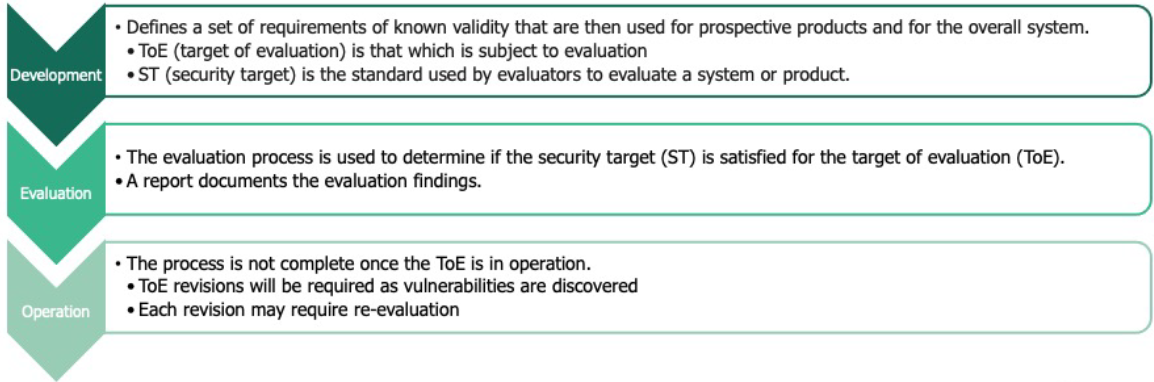
\includegraphics[width=\linewidth]{../img/common_criteria.png}
\textbf{Assurance Levels (EAL:}\\
\begin{itemize}
    \item EAL 1: Functionally tested
    \item EAL 2: Structurally tested
    \item EAL 3: Methodically tested and Checked
    \item EAL 4: Methodically Designed, Tested and Reviewed
    \item EAL 5: Semiformal Designed, and Tested
    \item EAL 6: Semiformal Verified Design and Tested
    \item EAL 7: Formally Verified Design and Tested
\end{itemize}

\subsubsection{CC Evaluation}
\begin{enumerate}
    \item Protection Profile
    \begin{itemize}
        \item Implementation independant, domain specific set of security requirements
    \end{itemize}
    \item Security Target
    \begin{itemize}
        \item Specific requirements used to evaluate system
    \end{itemize}
\end{enumerate}

\subsubsection{Example Threat in CC}
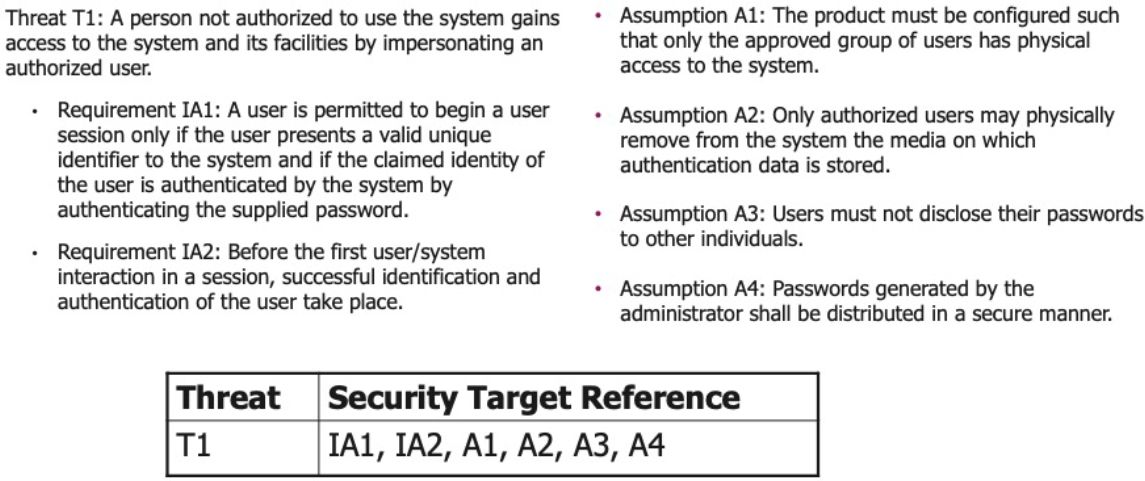
\includegraphics[width=\linewidth]{../img/example_threat_cc.png}
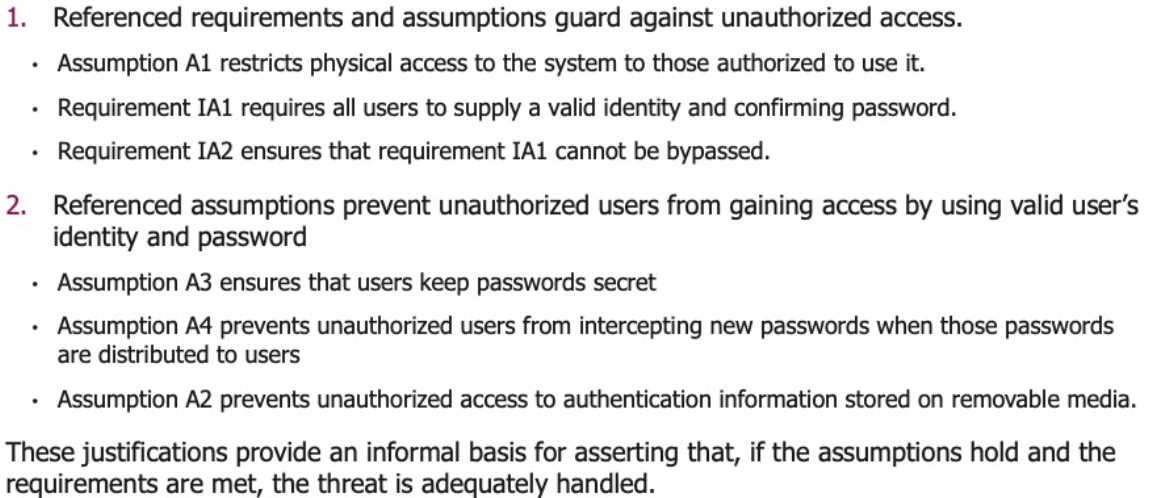
\includegraphics[width=\linewidth]{../img/example_threat_cc2.png}

\subsection{Security Target}
\subsubsection{PP/ST Framework}
\begin{itemize}
    \item Product Approach usually for STs
    \item Define what product does
    \item Define existing documentation/assurance
\end{itemize}
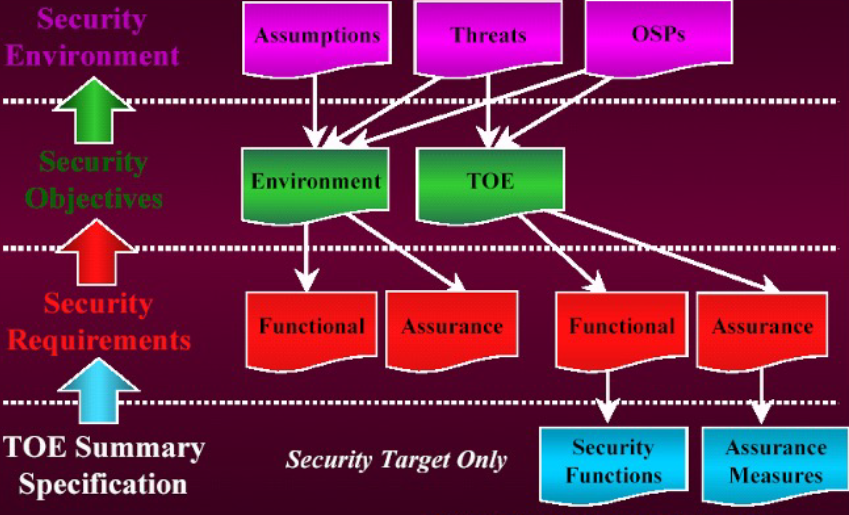
\includegraphics[width=0.5\linewidth]{../img/pp_st_framework.png}
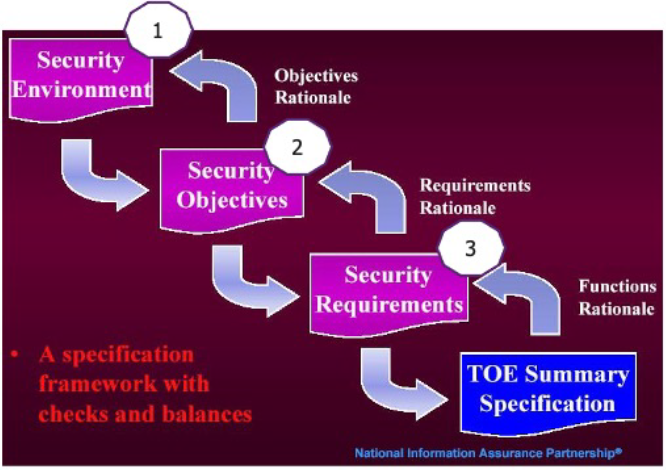
\includegraphics[width=0.5\linewidth]{../img/pp_st_framework2.png}

\subsubsection{Security Environment}
\begin{itemize}
    \item \textbf{Secure usage Assumptions} aspects of the environment intended to use
    \item Describes the security aspects
    \item \textbf{Threats:} The ability to exploit a vulnerability by a threat agent
    \item \textbf{Organizational Security Policies:} Set of rules, procedures, practices imposed by an organization
\end{itemize}

\subsubsection{Security Requirements}
\textbf{Functional Requirements}
\begin{itemize}
    \item Defining security behaviour
    \item Implemented requirements become security functions
    \item Examples:
    \begin{itemize}
        \item Identification / Authentication
        \item Audit
        \item User Data protection
    \end{itemize}
\end{itemize}
\textbf{Assurance Requirements}
\begin{itemize}
    \item Establishing confidence in security functions
    \begin{itemize}
        \item Correctness of implementation
        \item Effectiveness in satisfying security objectives
    \end{itemize}
    \item Examples:
    \begin{itemize}
        \item Development
        \item Configuration Management
        \item Life Cycle Support
        \item Testing
    \end{itemize}
\end{itemize}

\subsubsection{Reading Guidance}
\begin{itemize}
    \item Class: Differ in coverage of security objectives
    \item Family: Differ in rigor or emphasis
    \item Component: Describes an actual set of security requirements
    \item Element: Members of a component
\end{itemize}
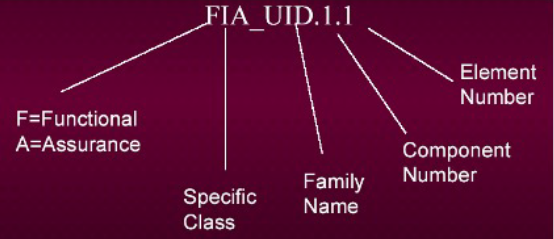
\includegraphics[width=0.6\linewidth]{../img/reading_guidance.png}

\subsubsection{Security Functionality Classes}
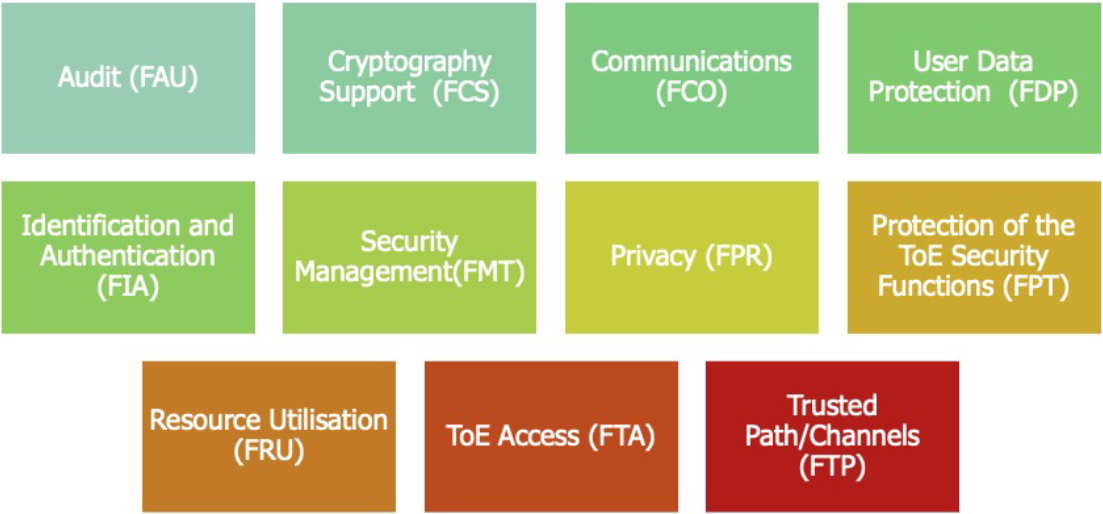
\includegraphics[width=\linewidth]{../img/security_functionality_classes.png}

\subsection{Design Document}
\begin{itemize}
    \item Provide basis for analysis
    \begin{itemize}
        \item Informal
        \item Semiformal
        \item Formal
    \end{itemize}
    \item Must include:
    \begin{itemize}
        \item Security Functions
        \item External Interfaces
        \item Internal Design
    \end{itemize}
\end{itemize}

\subsubsection{Security Functions}
\begin{itemize}
    \item Identifies high-level security functions defined for the system
    \item Includes:
    \begin{itemize}
        \item Description of individual functions
        \item Overview of set of security functions, how they work together
        \item Mapping of requirements, mapping functions to requirements
    \end{itemize}
\end{itemize}

\subsubsection{External Interfaces}
High level description of external interfaces to system, component, subcomponent or module
\begin{enumerate}
    \item \textbf{Component overview}: Identifying the component, its parent, how it fits into the design
    \item \textbf{Data descriptions:} Identifying data types and structures needed to support the external interface
    \item \textbf{Interface descriptions}
\end{enumerate}
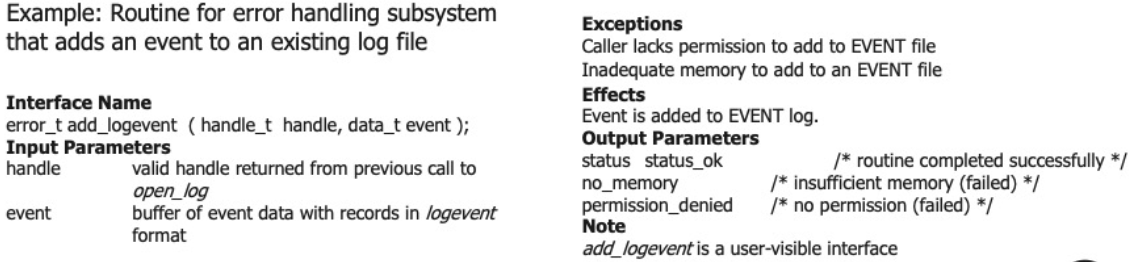
\includegraphics[width=\linewidth]{../img/external_interface.png}

\subsubsection{Internal Design}
Describes internal structures and functions of components of system.
\begin{enumerate}
    \item Overview of the parent component
    \item Detailed description of the component
    \item Security relevance of the component
\end{enumerate}

\subsection{Activities done to gain assurance}
\begin{enumerate}
    \item Analysis of the correspondence between TOE design representations
    \item Analysis of the TOE design representations against the requirements
    \item Analysis of functional tests coverage and results
    \item Independent functional testing
    \item Penetration testing
    \item Verification of mathematical proofs
    \item Analysis of guidance documents
    \item Analysis of processes and procedures
    \item Checking that processes and procedures are being applied
\end{enumerate}